\section{Preliminaries} \label{sec:preliminaries}

%We define boolean domain $\B = \{ \bot, \top \}$ as the set of boolean truth values, where $\bot < \top$ and they 
%complement each other, i.e., $\overline{\bot} = \top$ and $\overline{\top} = \bot$.
%
We denote by $\B = \{ \top, \bot \}$ the set of Booleans, $\R$ the set of reals, $\R_{\geq 0}$ the set of nonnegative reals, and $\R_{> 0}$ the 
set of positive reals.
%
An interval $I \subseteq \R$ of reals with the end points $a < b$ has length $|b-a|$.

Let $\Sigma$ be a finite {\em alphabet}.
%
We denote by $\Sigma^*$ the set of finite words over $\Sigma$ and by $\epsilon$ the empty word.
%
For $u \in \Sigma^*$, we respectively write $\pfx(u)$ and $\sfx(u)$ for the sets of prefixes 
and suffixes of $u$.
%
We also let $\infx(u) = \{v \in \Sigma^* \st \exists x,y \in \Sigma^* : u = xvy\}$.
%
For a nonempty word $u \in \Sigma^*$ and $1 \leq i \leq |u|$, we denote by $u[i]$ the $i$th letter of $u$.
%, by $u[..i]$ the prefix of $u$ of length $i$, and by $u[i..]$ the suffix of $u$ of length $|u| - i + 1$. 
%
Given $u \in \Sigma^*$ and $\ell \geq 1$, we denote by $u^\ell$ the word obtained by concatenating $u$ by itself $\ell - 1$ times.
Moreover, given $L \subseteq \Sigma^*$, we define $\first(L) = \{ u[1] \st u \in L\}$ and $\last(L) = \{ u[|u|] \st u \in L\}$
For sets $L_1, L_2 \subseteq \Sigma^*$ of words, we let $L_1 \cdot L_2 = \{u \cdot v \st u \in L_1, v \in L_2\}$.
For tuples $(u_1, \ldots, u_m)$ and $(v_1, \ldots, v_m)$ of words, we let $(u_1, \ldots, u_m) \cdot (v_1, \ldots, v_m) = (u_1 v_1, \ldots, u_m v_m)$.

We define the function $\destutter : \Sigma^* \to \Sigma^*$ inductively.
For all $\sigma \in \Sigma \cup \{\epsilon\}$, let $\destutter(\sigma) = \sigma$.
For all $u \in \Sigma^*$ such that $u = \sigma_1 \sigma_2 v$ for some $\sigma_1,\sigma_2 \in 
\Sigma$ and $v \in \Sigma^*$, we define it as follows:

%\vspace{-1em}
%\small
\begin{equation*}
	\destutter(u) =
	\begin{cases}
		\destutter(\sigma_2 v) & \text{if } \sigma_1 = \sigma_2 \\
		\sigma_1 \cdot \destutter(\sigma_2 v) & \text{otherwise}
	\end{cases}
\end{equation*}
%\normalsize
%For all $\sigma \in \Sigma \cup \{\epsilon\}$, let $\destutter(\sigma) = \sigma$.
%%
%For all $u \in \Sigma^*$ such that $u = \sigma_1 \sigma_2 v$ for some $\sigma_1,\sigma_2 \in 
%\Sigma$ and $v \in \Sigma^*$, let (i) $\destutter(u) = \destutter(\sigma_2 v)$ if $\sigma_1 = 
%\sigma_2$, and (ii) $\destutter(u) = \sigma_1 \cdot \destutter(\sigma_2 v)$ otherwise.
%%
For a set $L \subseteq \Sigma^*$ of finite words, we define $\destutter(L) = 
\{\destutter(u) \st u \in L\}$.
%
We extend $\destutter$ to tuples of words in a synchronized manner: for all $\sigma \in \Sigma \cup \{\epsilon\}$  let $\destutter(\sigma, \ldots, \sigma) = (\sigma, \ldots, \sigma)$.
Given a tuple $(u_1, \ldots, u_m) = (\sigma_{1,1} \sigma_{1,2} v_1, \ldots, \sigma_{m,1} \sigma_{m,2} v_m)$ of words of the same length, $\destutter(u_1, \ldots, u_m)$ is defined as expected:

%\vspace{-1em}
%\small
\begin{align*}
	&\destutter(u_1, \ldots, u_m) = \\
	&\begin{cases}
		\destutter(\sigma_{1,2} v_1, \ldots, \sigma_{m,2} v_m) \text{ if $\sigma_{i,1} = \sigma_{i,2}$ for}\\ 
		\hspace{14em}\text{all $1 \leq i \leq m$} \\
		(\sigma_{1,1}, \ldots, \sigma_{m,1}) \cdot \destutter(\sigma_{1,2} v_1, \ldots, \sigma_{m,2} v_m) \\
		\hspace{15.5em}\text{otherwise}
	\end{cases}
\end{align*}
%\normalsize
%Given a tuple $(u_1, \ldots, u_m) = (\sigma_{1,1} \sigma_{1,2} v_1, \ldots, \sigma_{m,1} \sigma_{m,2} v_m)$ of finite words of the same length, we define $\destutter(u_1, \ldots, u_m)$ as expected: (i) $\destutter(u_1, \ldots, u_m) = \destutter(\sigma_{1,2} v_1, \ldots, \sigma_{m,2} v_m)$ if $\sigma_{i,1} = 
%\sigma_{i,2}$ for all $1 \leq i \leq m$, and (ii) $\destutter(u_1, \ldots, u_m) = (\sigma_{1,1}, \ldots, \sigma_{m,1}) \cdot \destutter(\sigma_{1,2} v_1, \ldots, \sigma_{m,2} v_m)$ otherwise.

Moreover, given an integer $k \geq 0$, we define $\stutter_k : \Sigma^* \to \Sigma^*$ such that $\stutter_k(u) = \{v \in \Sigma^* \st |v| = k \land \destutter(v) = \destutter(u)\}$ if $k \geq |\destutter(u)|$, and $\stutter_k(u) = \emptyset$ otherwise.

\paragraph*{Signal Temporal Logic (STL) \cite{MalerN13}.}
%\noindent\textbf{Signal Temporal Logic (STL) \cite{MalerN13}.}
Let $A,B \subset \R$.
%
A function $f : A \to B$ is
\emph{right-continuous} iff $\lim_{a \to c^+} f(a) = f(c)$ for all $c \in A$, and
%\emph{left-limited} iff $\lim_{a \to c^-} f(a) < \infty$ for all $c \in A$;
\emph{non-Zeno} iff for every bounded interval $I \subseteq A$ there are finitely many $a \in I$ such that $f$ is not continuous at $a$.
%
A \emph{signal} is a right-continuous, non-Zeno, piecewise-constant function $x : [0,d) \to \R$ where $d \in \R_{> 0}$ is the duration of $x$ and $[0,d)$ is its temporal domain.
Let $x : [0,d) \to \R$ be a signal.
An \emph{event} of $x$ is a pair $(t, x(t))$ where $t \in [0,d)$.
An \emph{edge} of $x$ is an event $(t, x(t))$ such that $\lim_{s \to t^-} x(s) \neq \lim_{s \to t^+} x(s)$.
In particular, an edge is \emph{rising} if $\lim_{s \to t^-} x(s) < \lim_{s \to t^+} x(s)$, and it is \emph{falling} otherwise.
A signal $x : [0,d) \to \R$ can be represented finitely by its initial value and edges: if $x$ has $m$ edges, then $x = (t_0, v_0) (t_1, v_1) \ldots (t_m, v_m)$ such that $t_0 = 0$, $t_{i-1} < t_i$, and $(t_i, v_i)$ is an edge of $x$ for all $1 \leq i \leq m$.

\bgroup \color{red}
Let $\AP$ be a set of \emph{atomic propositions}.
The syntax of \emph{future STL} is given by the grammar $\varphi :=  p ~|~ \lnot \varphi ~|~ \varphi \land \varphi ~|~ \varphi \until_I \varphi$ and that of \emph{past STL} is given by $\varphi :=  p ~|~ \lnot \varphi ~|~ \varphi \land \varphi ~|~ \varphi \since_I \varphi$ where $p \in \AP$ and $I \subseteq \R_{\geq 0}$ is an interval.
Below, when we speak of an STL formula, we mean either a future STL or a past STL formula.

A \emph{trace} $w = (x_1, \ldots, x_n)$ is a finite vector of signals.
We express atomic propositions as functions of trace values at a time point $t$,
i.e., a proposition $p \in \AP$ over a trace $w = (x_1, \ldots, x_n)$ is defined as $f_p(x_1(t), \ldots, x_n(t)) > 0$ where $f_p : \R^n \to \R$ is a function.
%i.e., a proposition $p \in \AP$ over a trace $w = (x_1, \ldots, x_n)$ is defined as $f_p(x_1(t), \ldots, x_n(t)) \sim_p c_p$ where $f_p : \R^n \to \R$ is a function, $c_p \in \R$ is a constant, and ${\sim_p} \in \{{<}, {\leq}, {\geq}, {>}\}$.
Given intervals $I,J \subseteq \R_{\geq 0}$, we define $I \oplus J = \{i + j \st i \in I , j \in J\}$ and $I \ominus J = \{i - j \st i \in I , j \in J\}$, where we simply write $t$ for the singleton set $\{t\}$. 

We recall the finite-trace qualitative semantics of STL defined over $\B$.
Let $d \in \R_{> 0}$ and $w = (x_1, \ldots, x_n)$ with $x_i : [0,d) \to \R$ for all $1 \leq i \leq n$.
Let $\varphi_1, \varphi_2$ be STL formulas and let $t \in [0,d)$.

%\small
\begin{align*}
	(w,t) \models p \iff & f_p(x_1(t), \ldots, x_n(t)) > 0 \\
	(w,t) \models \lnot \varphi_1 \iff & \overline{(w,t) \models \varphi_1} \\
	(w,t) \models \varphi_1 \land \varphi_2 \iff & (w,t) \models \varphi_1 \land (w,t) \models \varphi_2 \\
	(w,t) \models \varphi_1 \until_I \varphi_2 \iff & \exists t' \in (t \oplus I) \cap [0,d) :  \\
	& (w,t') \models \varphi_2 \land \forall t'' \in (t, t') : \\
	& (w,t'') \models \varphi_1\\
	(w,t) \models \varphi_1 \since_I \varphi_2 \iff & \exists t' \in (t \ominus I) \cap [0,d) :  \\
	& (w,t') \models \varphi_2 \land \forall t'' \in (t', t) : \\
	& (w,t'') \models \varphi_1
\end{align*}
%\normalsize

When $\varphi$ is a future (resp. past) STL formula, we simply write $w \models \varphi$ for $(w,0) \models \varphi$ (resp. $(w,d) \models \varphi$).
We additionally use the following standard abbreviations: 
$\false = p \land \lnot p$,
$\true = \lnot \false$,
$ \varphi_1 \lor \varphi_2 = \lnot (\lnot \varphi_1 \land \lnot \varphi_2)$,
$\LTLf_I \varphi = \true \until_I \varphi$,
$\LTLg_I \varphi = \lnot \LTLf_I \lnot \varphi$,
$\LTLdiamondminus_I \varphi = \true \since_I \varphi$, and
$\LTLsquareminus_I \varphi = \lnot \LTLdiamondminus_I \lnot \varphi$.
Moreover, the untimed temporal operators are defined through their timed counterparts on the interval $[0,\infty)$.

Future STL formulas whose timed operators are bounded (i.e., use of $\until_I$ is restricted to intervals $I$ with a real-valued right end point) can be translated to past STL formulas, which can be monitored efficiently in an online manner~\cite{MalerNP07,JaksicBGKNN15,Gol18}.
\egroup

\paragraph*{Distributed Semantics of STL \cite{MomtazAB23}.}
%\noindent\textbf{Distributed Semantics of STL \cite{MomtazAB23}.}
We consider an asynchronous and loosely-coupled message-passing system of $n \geq 2$ reliable agents producing a set of signals $x_1, \ldots, x_n$, where for some $d \in \R_{> 0}$ we have $x_i : [0,d) \to \R$ for all $1 \leq i \leq n$.
%
The agents do not share memory or a global clock.
%
Only to formalize statements, we speak of a \emph{hypothetical} global clock and denote its value by $T$.
%
For local time values, we use the lowercase letters $t$ and $s$.
For a signal $x_i$, we denote by $V_i$ the set of its events, and by $E_i$ the set of its edges.
%For a signal $x_i$, we denote by $V_i$ the set of its events, by $E_i^\uparrow$ the set of its rising edges, and by $E_i^\downarrow$ that of falling edges.
%Moreover, we let $E_i = E_i^\uparrow \cup E_i^\downarrow$.
%
We represent the local clock of the $i$th agent as an increasing and divergent function $c_i : 
\R_{\geq 0} \to \R_{\geq 0}$ that maps a global time $T$ to a local time $c_i(T)$.

We assume that the system is \emph{partially synchronous}: the agents use a clock synchronization algorithm that guarantees a bounded clock skew with respect to the global clock, i.e., $|c_i(T) - c_j(T)| < \varepsilon$ for all $1 \leq i,j \leq N$ and $T \in \R_{\geq 0}$, where $\varepsilon \in \R_{> 0}$ is the maximum clock skew.

\begin{definition} \label{defn:hb}
	A \emph{distributed signal} is a pair $(S, {\hb})$, where $S = (x_1, \ldots, x_n)$ is a vector of 
	signals and ${\hb}$ is the happened-before relation between events defined as follows:
	(1) For every agent, the events of its signals are totally ordered, i.e., for all $1 \leq i \leq n$ and all $(t, x_i(t)), (t', x_i(t')) \in V_i$, if $t < t'$ then $(t, x_i(t)) \hb (t', x_i(t'))$.
	(2) Every pair of events whose timestamps are at least $\varepsilon$ apart is totally ordered, i.e., for all $1 \leq i,j \leq n$ and all $(t, x_i(t)) \in V_i$ and $(t', x_j(t')) \in V_j$, if $t + \varepsilon \leq t'$ then $(t, x_i(t)) \hb (t', x_j(t'))$.
\end{definition}

The notion of \emph{consistent cut} captures possible global states.

\begin{definition}
	Let $(S, {\hb})$ be a distributed signal of $n$ signals, and $V = \bigcup_{i = 1}^{n} V_i$ be the set of its events.
	A set $C \subseteq V$ is a \emph{consistent cut} iff for every event in $C$, all events that happened before  it also belong to $C$, i.e., for all $e, e' \in V$, if $e \in C$ and $e' \hb e$, then $e' \in C$.
\end{definition}

We denote by $\CC(T)$ the set of consistent cuts at global time $T$.
Given a consistent cut $C$, its \emph{frontier} $\fr(C) \subseteq C$ is the set consisting of the last events in $C$ of each signal, i.e., $\fr(C) = \bigcup_{i = 1}^{n} \{ (t, x_i(t)) \in V_i \cap C \st \forall t' > t : (t', x_i(t')) \notin V_i \cap C \}$.

\begin{definition}
A \emph{consistent cut flow} is a function $\ccf : \R_{\geq 0} \to 2^V$ that maps a global clock value $T$ to the frontier of a consistent cut at time $T$, i.e., $\ccf(T) \in \{\fr(C) \st C \in \CC(T)\}$.
\end{definition}

\begin{figure}{r}
	%	\vspace{-3em}
	\centering
	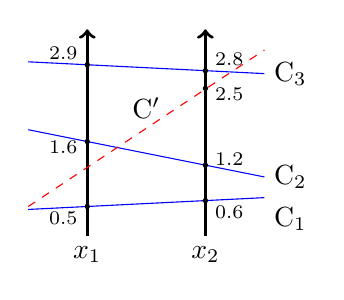
\begin{tikzpicture}[scale=0.75]
		% Draw the arrows
		\draw[very thick, ->] (0,0) node[below] {$x_1$} -- (0,3.5) ;
		\draw[very thick, ->] (2,0) node[below] {$x_2$} -- (2,3.5) ;
		
		% Draw the lines with labels extended further left and right
		\draw[blue] (-1,0.45) -- (3,0.65) node[right, below right, black] {C$_1$};
		\draw[blue] (-1,1.8) -- (3,1.0) node[right, black] {C$_2$};
		\draw[blue] (-1,2.95) -- (3,2.75) node[right, black] {C$_3$};
		
		% Dashed line extended further left and right
		\draw[red, dashed] (-1,0.5) -- (3,3.15) node[midway, above, black] {C$'$};
		
		% Labels on the left arrow with markers
		\node[left] at (0,0.3) {{\scriptsize 0.5}};
		\node[left] at (0,1.5) {{\scriptsize 1.6}};
		\node[left] at (0,3.1) {{\scriptsize 2.9}};
		\draw[fill=black] (0,0.5) circle (1pt);
		\draw[fill=black] (0,1.6) circle (1pt);
		\draw[fill=black] (0,2.9) circle (1pt);
		
		% Labels on the right arrow with markers
		\node[right] at (2,0.4) {{\scriptsize 0.6}};
		\node[right] at (2,1.3) {{\scriptsize 1.2}};
		\node[right] at (2,2.4) {{\scriptsize 2.5}};
		\node[right] at (2,3.0) {{\scriptsize 2.8}};	
		\draw[fill=black] (2,0.6) circle (1pt);
		\draw[fill=black] (2,1.2) circle (1pt);
		\draw[fill=black] (2,2.5) circle (1pt);
		\draw[fill=black] (2,2.8) circle (1pt);
	\end{tikzpicture}
	\caption{A distributed signal in with consistent cuts $C_1, C_2, C_3$ constituting a consistent cut flow. Note that $C'$ is a non-example since $(2.5, x_2(2.5)) \in \fr(C')$~and $(1.6, x_1(1.6)) \notin \fr(C')$,~but  $(1.6, x_1(1.6))$~happened
		before~$(2.5, x_2(2.5))$.} \label{fig:distsig}
	%	\vspace{1em}
\end{figure}

For all $T,T' \in \R_{\geq 0}$ and $1 \leq i \leq n$, if $T < T'$, then for every pair of events $(c_i(T), x_i(c_i(T))) \in \ccf(T)$ and $(c_i(T'), x_i(c_i(T'))) \in \ccf(T')$ we have $(c_i(T), x_i(c_i(T))) \hb (c_i(T'), x_i(c_i(T')))$.
We denote by $\CCF(S,{\hb})$ the set of all consistent cut flows of the distributed signal $(S,{\hb})$.


%\begin{example} \label{ex:distsig}
%	Let $(S,{\hb})$ be a distributed signal with $S = (x_1, x_2)$ and $\varepsilon = 0.5$, where some events of $x_1$ and $x_2$ are marked on \cref{fig:distsig}.
%	For example, $(0.5, x_1(0.5)) \hb (1.6, x_1(1.6)) \hb (2.5, x_2(2.5)) \hb (2.8, x_2(2.8))$, but $(2.5, x_2(2.5)) \not\hb (2.9, x_1(2.9))$.
%	The solid blue lines marked with $C_1, C_2, C_3$ correspond to a consistent cut, e.g., $\fr(C_3) = \{(2.9, x_1(2.9)), (2.8, x_2(2.8))\}$, however $C'$ is not a consistent cut since $(2.5, x_2(2.5)) \in \fr(C')$ and $(1.6, x_1(1.6)) \hb (2.5, x_2(2.5))$ but $(1.6, x_1(1.6)) \notin \fr(C')$.
%	Moreover, the frontiers of these consistent cuts can be seen as produced by a consistent cut flow $\ccf$, e.g., with $\ccf(0.5) = \fr(C_1)$, $\ccf(1) = \fr(C_2)$, and $\ccf(2) = \fr(C_3)$.	
%\end{example}

%\begin{wrapfigure}{r}{0.3\textwidth}
%	\vspace{-2em}
%	\begin{center}
%		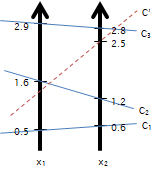
\includegraphics[scale=0.9]{distsig.png}
%	\end{center}
%	\caption{The distributed signal in \cref{ex:distsig} with consistent cuts $C_1, C_2, C_3$}
%	\label{fig:distsig}
%\end{wrapfigure}



Observe that a consistent cut flow of a distributed signal induces a vector of synchronous signals which can be evaluated using the standard STL semantics described above.
Let $(S,{\hb})$ be a distributed signal of $n$ signals $x_1, \ldots, x_n$.
A consistent cut flow $\ccf \in \CCF(S,{\hb})$ yields a trace $w_{\ccf} = (x'_1, \ldots x'_n)$ on the temporal domain $[0,d)$ such that $(c_i(T), x_i(c_i(T))) \in \ccf(T)$ implies $x_i'(T) = x_i(c_i(T))$ for all $1 \leq i \leq n$ and $T \in [0, d)$.
The set of traces of $(S,{\hb})$ is given by $\tr(S,{\hb}) = \{ w_{\ccf} \st \ccf \in \CCF(S,{\hb})\}$.

We define the satisfaction of an STL formula $\varphi$ by a distributed signal $(S,{\hb})$ over a three-valued domain $\{\top, \bot, {?}\}$
%If the set of synchronous traces $\tr(S,{\hb})$ defined by a distributed signal $(S,{\hb})$ is contained in the set of traces allowed by the formula $\varphi$, then $(S,{\hb})$ satisfies $\varphi$.
%Similarly, if $\tr(S,{\hb})$ has an empty intersection with the set of traces $\varphi$ defines, then $(S,{\hb})$ violates $\varphi$.
%Otherwise, the evaluation is inconclusive since some traces satisfy the property and some violate it.
Notice that we quantify universally over traces for both satisfaction and violation.

%\vspace{-1em}
%\footnotesize
\begin{equation*}
	[(S,{\hb}) \models \varphi] = 
	\begin{cases}
		\top \text{ if } \forall w \in \tr(S,{\hb}) : w \models \varphi \\
		\bot \text{ if } \forall w \in \tr(S,{\hb}) : w \models \lnot\varphi \\
		\,?\, \text{ otherwise}
	\end{cases}
\end{equation*}
%\normalsize



\section{Overapproximation of the STL Distributed Semantics}
\label{sec:semantics}

To address the computational overhead in exact distributed monitoring, we define STL$^+$, a variant of STL whose syntax is the same as STL but semantics provide a sound approximation of the STL distributed semantics.
In particular, given a distributed signal $(S,{\hb})$, STL$^+$ considers an approximation 
$\tr^+(S,{\hb})$ of the set $\tr(S,{\hb})$ of synchronous traces where $ \tr(S,{\hb}) \subseteq \tr^+(S,{\hb})$.
A signal $(S,{\hb})$ satisfies (resp. violates) an STL$^+$ formula $\varphi$ iff all the traces in $\tr^+(S,{\hb})$ belong to the language of $\varphi$ (resp. $\lnot \varphi$).

%\vspace{-1em}
%\footnotesize
\begin{equation*}
	[(S,{\hb}) \models \varphi]_+ = 
	\begin{cases}
		\top \text{ if } \forall w \in \tr^+(S,{\hb}) : w \models \varphi \\
		\bot \text{ if } \forall w \in \tr^+(S,{\hb}) : w \models \lnot\varphi \\
		\,?\, \text{ otherwise}
	\end{cases}
\end{equation*}
%\normalsize

%%% this may be not wlog -- the verdict may change when a formula is made copyless
Throughout the paper, we assume  $\varphi$ is \emph{copyless}, i.e., each signal $x \in S$ occurs in $\varphi$ at most once.
Moreover, the signals are Boolean, non-Zeno, piecewise-constant, and have no edge at time 0.
We assume Boolean signals only for convenience; all the concepts and results generalize to non-Boolean signals because finite-length piecewise-constant signals use only a finite number of values.
We note that our approach is a sound overapproximation also for non-copyless formulas, although potentially less precise.


In \cref{sec:approach}, we define $\tr^+$ show that it overapproximates $\tr$ (\cref{cl:trsound}), which implies the soundness of STL$^+$ as stated in \cref{cl:stlsound}.
In \cref{sec:algorithm} we present algorithm to compute the semantics of STL$^+$ and extend it to online monitoring.

\begin{theorem} \label{cl:stlsound}
	Consider a distributed signal $(S,{\hb})$ and an STL formula $\varphi$.
	The following implications hold:
	\begin{align*}
		[(S,{\hb}) \models \varphi]_+ = \top &\implies [(S,{\hb}) \models \varphi] = \top \\
		[(S,{\hb}) \models \varphi]_+ = \bot &\implies [(S,{\hb}) \models \varphi] = \bot \\
	\end{align*}
\end{theorem}
\begin{proof}[\normalsize Proof.]
	\normalsize
	Let $\varphi$ be an STL formula and $(S,{\hb})$ be a distributed signal.
	Assume $[(S,{\hb}) \models \varphi]_+ = \top$.
	We want to show that $[(S,{\hb}) \models \varphi] = \top$.
	Expanding the definition of $[(S,{\hb}) \models \varphi]_+ = \top$, we have $w \models \varphi$ for all $w \in \tr^+(S,{\hb})$.
	By \cref{cl:trsound}, we have $\tr(S,{\hb}) \subseteq \tr^+(S,{\hb})$.
	Then, it holds that $w \models \varphi$ for all $w \in \tr(S,{\hb})$.
	Therefore, $[(S,{\hb}) \models \varphi] = \top$ by definition.
	The case of $[(S,{\hb}) \models \varphi]_+ = \bot$ follows from the same arguments.
\end{proof}


Notice that both the distributed semantics of STL and the semantics of STL$^+$ quantify universally over the set of traces for the verdicts $\top$ and $\bot$.
Therefore, \cref{cl:stlsound} holds for the verdicts $\top$ and $\bot$, but not for ${\,?}$.

